\section{Experimentación}

Queremos ver empíricamente que las complejidades de los algoritmos es la cota teórica demostrada en la sección de desarrollo. Para esto se diseñaron una serie de tests que fueron generados con el programa \textit{generatetest.py}. En estos, el ángulo fue fijado en $10$, y el radio ($m$) fue variando entre $5$ y $80$.
Cada archivo de test tiene $40$ instancias en las que los valores de las paredes internas y externas son aleatorios y varían en un determinado valor respecto de los valores adyacentes. Estos mismos archivos de entrada son los que usamos para generar los gráficos que aparecen a continuación, para medir distintos tiempos de ejecución con uno u otro método, en nanosegundos o milisegundos.

Como lo que nos interesa medir es el tiempo de ejecución y éste depende del tamaño de la matriz, con variar $n$ ó $m$ ya basta para ver como aumentan los tiempos en función del tamaño.

Los tests fueron corridos todos en una CPU Intel I5-760 de 2.80 Ghz. Los tiempos varían de acuerdo a la máquina, pero lo que nos interesa es hacer la comparación y ver la manera en que crecen.

Medimos para cada test el tiempo total en resolver las 40 instancias, para evitar que la presencia de $outliers$ influyera de manera significativa en los tiempos de ejecución. No tuvimos en cuenta los tiempos de carga de las matrices y vectores, ni de la salida de los resultados.

Para obtener el siguiente gráfico, lo que hicimos fue dividir el tiempo de ejecución por $m^{2}$, para de esta manera obtener el gráfico de una recta y probar efectivamente que el tiempo de ejecución real del algoritmo de Eliminación Gaussiana es el dicho en la sección anterior.

\begin{figure}[h]
  \center
  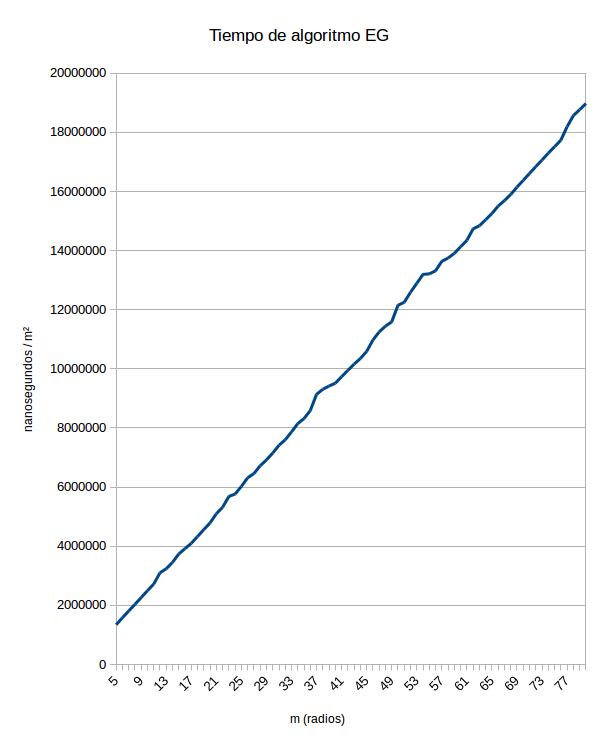
\includegraphics[scale=0.8]{imagenes/tiempoEGdivididoM2.png}
  %\caption{La figura}
  \label{fig:egdivididom2}
\end{figure}

En el gráfico a continuación, lo que hicimos fue considerar 2 casos: contamos el tiempo de obtención de las matrices L y U, y luego no lo contamos. En ambos casos dividimos el tiempo de ejecución por $m$. En el primer caso, al dividir por $m$, el gráfico crece de manera parabólica, ya que el tiempo que tarda el algoritmo en obtener las matrices L y U es cúbico respecto del tamaño de la matriz. Por lo tanto, al dividir por m, el tiempo de ejecución debería crecer de forma cuadrática, lo cual se puede observar en el gráfico. 


\begin{figure}[h]
  \center
  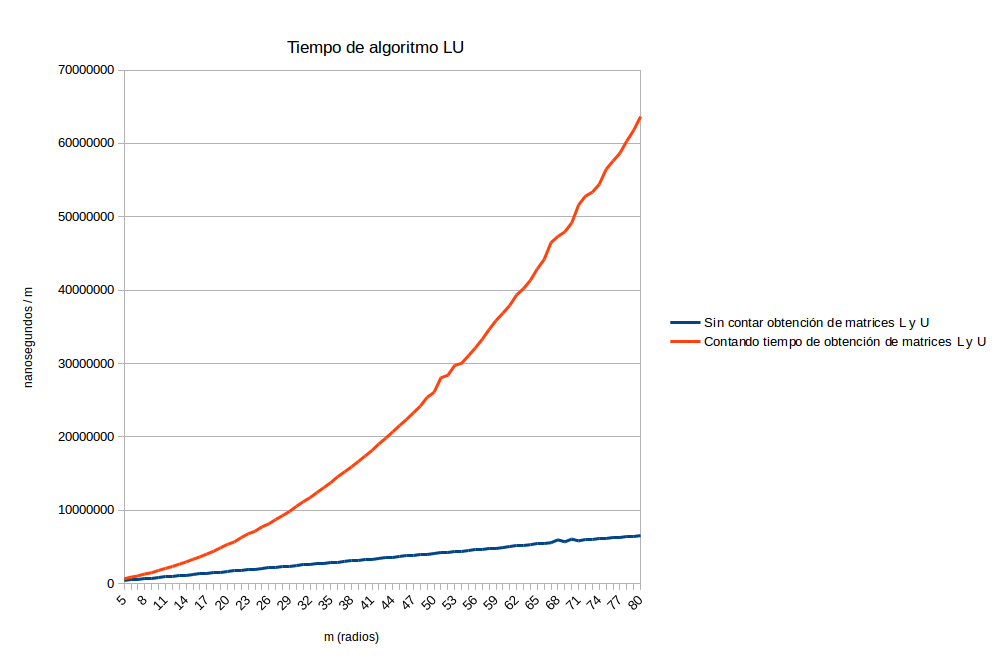
\includegraphics[scale=0.6]{imagenes/tiempoLUdivididoM.png}
  %\caption{La figura}
  \label{fig:ludivididom}
\end{figure}


En el segundo caso no se tuvo en cuenta el tiempo de obtención de las matrices L y U, por lo tanto el tiempo de ejecución del algoritmo es cuadrático, y al dividir todo por $m$, obtenemos una recta, como se puede observar. \\


Por último vamos a comparar directamente el tiempo de ejecución de la eliminación gaussiana contra el tiempo de ejecución de LU (contando el tiempo de obtención de la matriz LU). En este caso los tiempos de ejecución no fueron divididos por $m$ ya que solamente queríamos poder comparar a grandes rasgos las diferencias entre los tiempos de ejecución de ambos algoritmos. Por más que ambos algoritmos tienen complejidad cúbica, se puede observar que la eliminación gaussiana toma considerablemente más tiempo, lo cual nos confirma empíricamente la importancia de guardarnos las matrices L y U a la hora de resolver un sistema de ecuaciones.

\newpage

\begin{figure}[h]
  \center
  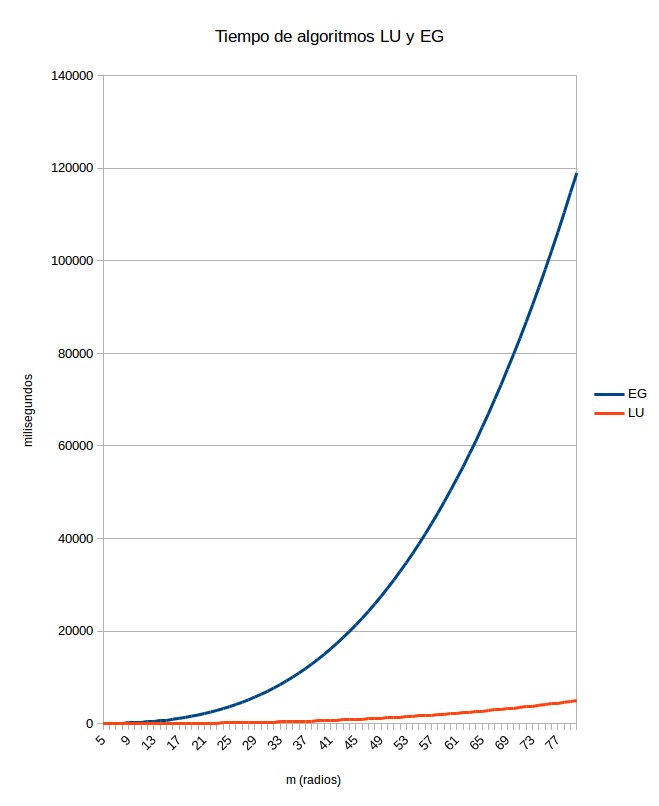
\includegraphics[scale=0.8]{imagenes/tiempoLUyEGsinDividir.png}
  %\caption{La figura}
  \label{fig:luyeg}
\end{figure}

